\chapter{Dimensionality Reduction and Principal Component Analysis}
\label{ch:dimred}
\newcommand{\irisPAplot}{\addplot[only marks,mlblue,mark=*,mark size=2pt] coordinates {(-2.68,0.32) (-2.89,-0.14) (-2.73,0.33) (-2.82,-0.09) (-2.89,-0.58) (-2.51,0.65) (-2.79,-0.24) (-2.64,1.18) (-2.62,0.81) (-2.20,0.87) (-2.31,0.39) (-3.22,0.13) (-2.36,-0.04) (-2.47,0.13) (-2.64,0.31) (-2.59,-0.20) (-2.65,0.81) (-2.64,-0.12) (-2.63,0.60) (-2.98,-0.49) (-2.77,0.26) (-3.00,-0.34) (-2.21,0.44) (-2.54,0.50) (-2.54,0.58)};}
\newcommand{\irisPBplot}{\addplot[only marks,mlorange,mark=triangle*,mark size=2.6pt] coordinates {(1.28,0.69) (1.46,0.50) (1.09,0.07) (1.10,0.28) (1.04,0.23) (-0.51,-1.27) (0.26,-0.55) (-0.17,-0.25) (0.66,-0.35) (0.94,-0.54) (1.12,-0.08) (1.30,-0.33) (0.71,0.15) (1.33,0.24) (0.81,-0.16) (-0.07,-0.71) (0.14,-0.31) (0.59,-0.48) (1.22,0.41) (0.25,-0.27) (0.46,-0.67) (0.23,-0.40) (0.36,-0.50) (0.38,-0.29) (-0.91,-0.76)};}
\newcommand{\irisPCplot}{\addplot[only marks,mlgreen,mark=square*,mark size=2pt] coordinates {(2.53,-0.01) (2.62,0.34) (2.35,-0.04) (0.52,-1.19) (2.32,-0.24) (1.66,0.24) (2.17,0.22) (1.59,-0.54) (1.95,0.04) (3.80,0.26) (2.43,0.38) (3.50,0.46) (2.28,0.33) (1.26,-0.18) (2.12,-0.21) (2.84,0.38) (2.16,-0.22) (1.78,-0.50) (2.14,0.14) (1.17,-0.16) (2.31,0.18) (1.42,-0.57) (2.42,0.30) (1.53,-0.38) (1.90,0.12)};}

\newcommand{\digitscumplot}{\addplot[very thick,mlblue,mark=*,mark size=1.2pt] coordinates {(1,0.1489) (2,0.2851) (3,0.4030) (4,0.4871) (5,0.5450) (6,0.5941) (7,0.6373) (8,0.6739) (9,0.7074) (10,0.7382) (11,0.7620) (12,0.7847) (13,0.8029) (14,0.8206) (15,0.8353) (16,0.8494) (17,0.8626) (18,0.8751) (19,0.8852) (20,0.8943) (21,0.9032) (22,0.9112) (23,0.9188) (24,0.9261) (25,0.9330) (26,0.9390) (27,0.9447) (28,0.9499) (29,0.9548) (30,0.9591) (31,0.9628) (32,0.9664) (33,0.9697) (34,0.9730) (35,0.9761) (36,0.9790) (37,0.9816) (38,0.9839) (39,0.9861) (40,0.9882) (41,0.9901) (42,0.9917) (43,0.9932) (44,0.9946) (45,0.9958) (46,0.9968) (47,0.9978) (48,0.9986) (49,0.9991) (50,0.9995) (51,0.9998) (52,0.9998) (53,0.9999) (54,0.9999) (55,1.0000) (56,1.0000) (57,1.0000) (58,1.0000) (59,1.0000) (60,1.0000) (61,1.0000) (62,1.0000) (63,1.0000) (64,1.0000)};}
\newcommand{\digitsscreeplot}{\addplot[very thick,mlpurple,mark=*,mark size=1.2pt] coordinates {(1,0.1489) (2,0.1362) (3,0.1179) (4,0.0841) (5,0.0578) (6,0.0492) (7,0.0432) (8,0.0366) (9,0.0335) (10,0.0308) (11,0.0237) (12,0.0227) (13,0.0182) (14,0.0177) (15,0.0147) (16,0.0141) (17,0.0132) (18,0.0125) (19,0.0102) (20,0.0091) (21,0.0089) (22,0.0080) (23,0.0077) (24,0.0072) (25,0.0070) (26,0.0060) (27,0.0058) (28,0.0052) (29,0.0049) (30,0.0043)};}


\begin{objectives}
After studying this chapter you will be able to:
\begin{itemize}
  \item explain the \textbf{curse of dimensionality} and its effects on distances, data requirements and learning algorithms;
  \item distinguish \textbf{projection} from \textbf{manifold learning} and name the main methods in each family;
  \item explain \textbf{Principal Component Analysis (PCA)} and carry it out \textbf{by hand}: covariance matrix, eigenvalues, eigenvectors, projection and reconstruction;
  \item use \textbf{explained variance} to choose the number of components;
  \item explain why \textbf{feature scaling} is essential for PCA;
  \item use PCA for \textbf{visualisation}, \textbf{compression} and \textbf{preprocessing};
  \item describe \textbf{Kernel PCA}, \textbf{Incremental PCA} and \textbf{Randomised PCA};
  \item answer 2-, 5- and 10-mark university questions on this part of Unit~IV.
\end{itemize}
\end{objectives}

\begin{pullquote}[--- often attributed to Albert Einstein]
Everything should be made as simple as possible, but no simpler.
\end{pullquote}

%====================================================================
\section{Why Reduce the Number of Features?}

Real datasets can have a huge number of features: a $64\times64$ photograph has $4096$ pixel values, a gene-expression record has tens of thousands of measurements, and a document may have thousands of word counts. Yet most of these numbers are redundant: neighbouring pixels are almost equal, many genes move together, and most words are rare.

\begin{definition}[: Dimensionality reduction]
\textbf{Dimensionality reduction} is the process of transforming data from a high-dimensional space $\R^{d}$ into a lower-dimensional space $\R^{m}$ ($m<d$) while \emph{keeping as much of the useful information as possible}. It is an \emph{unsupervised} technique: it uses only the features $\vect x$, not the labels.
\end{definition}

\paragraph{Why do we do it?}
\begin{itemize}
  \item \textbf{Visualisation:} humans can look at 2-D or 3-D plots, not at 50-D data.
  \item \textbf{Speed and memory:} fewer features make training and prediction faster.
  \item \textbf{Fighting the curse of dimensionality:} many learning algorithms perform worse as features are added (next section).
  \item \textbf{Removing noise and redundancy:} the discarded directions are often mostly noise.
  \item \textbf{Compression:} store 30 numbers instead of 64.
\end{itemize}

%====================================================================
\section{The Curse of Dimensionality}

\begin{definition}[: Curse of dimensionality]
The \textbf{curse of dimensionality} (a term coined by Richard Bellman) refers to the collection of problems that appear when the number of features $d$ becomes large: the volume of the space grows so fast that \emph{any fixed amount of data becomes extremely sparse}; distances between points become almost equal and therefore lose meaning; and the amount of data needed to learn reliably grows exponentially with $d$.
\end{definition}

\subsection{Cartoon: A Lonely Point in a Big Space}

Put the same ten points in a line, in a square and in a cube. In one dimension they crowd together and every point has many close neighbours. In three dimensions the same ten points are lost in a huge space.

\begin{figure}[!htbp]
\centering
\resizebox{\linewidth}{!}{%
\begin{tikzpicture}
% ---------------- 1-D ----------------
\node[font=\small\bfseries] at (1.8,4.4) {1 feature (a line)};
\draw[very thick] (0,0)--(3.6,0);
\foreach \x in {0.2,0.55,0.9,1.3,1.6,2.0,2.35,2.8,3.1,3.45} \fill[mlblue] (\x,0) circle (0.07);
\pic[scale=1.1] at (1.8,3.45) {smile};
\node[font=\footnotesize,align=center] at (1.8,-0.9) {neighbourhood of radius $0.1$\\covers \textbf{20\%} of the space};
% ---------------- 2-D ----------------
\begin{scope}[xshift=5.6cm]
\node[font=\small\bfseries] at (1.8,4.4) {2 features (a square)};
\draw[very thick] (0,-0.9) rectangle (3.2,2.3);
\foreach \x/\y in {0.3/0.1,1.0/1.9,2.4/0.5,0.7/0.9,2.0/1.6,2.9/2.0,1.5/-0.3,0.4/1.5,2.6/-0.5,1.6/0.8} \fill[mlblue] (\x,\y) circle (0.07);
\pic[scale=1.1] at (1.6,3.45) {meh};
\node[font=\footnotesize,align=center] at (1.6,-1.85) {neighbourhood of radius $0.1$\\covers \textbf{3.1\%} of the space};
\end{scope}
% ---------------- 3-D ----------------
\begin{scope}[xshift=11.2cm]
\node[font=\small\bfseries] at (1.8,4.4) {3 features (a cube)};
\draw[very thick] (0,-0.7) rectangle (2.4,1.7);
\draw[very thick] (0.8,0.0) rectangle (3.2,2.4);
\foreach \a/\b in {0/-0.7,2.4/-0.7,0/1.7,2.4/1.7} \draw[thick] (\a,\b)--(\a+0.8,\b+0.7);
\foreach \x/\y in {0.3/-0.2,1.8/1.2,1.0/0.5,2.6/1.9,2.9/0.9,0.5/1.3,2.0/-0.3,1.6/0.6,0.9/1.9,2.3/0.4} \fill[mlblue] (\x,\y) circle (0.07);
\pic[scale=1.1] at (1.6,3.45) {sad};
\node[font=\footnotesize,align=center] at (1.6,-1.65) {neighbourhood of radius $0.1$\\covers \textbf{0.42\%} of the space};
\end{scope}
\end{tikzpicture}}
\caption{The same ten points become more and more isolated as the number of dimensions grows.}\label{fig:sparse}
\end{figure}

\begin{explain}
In all three drawings there are exactly ten blue points, but the \textbf{space they live in grows}: a line, a square, a cube. The faces show how it feels to be a point. In 1-D a ball of radius $0.1$ around a point covers $20\%$ of the whole line, so a point is surrounded by friends (happy face). In 2-D the same radius covers only $\pi(0.1)^2=3.1\%$ of the square, so neighbours are rarer (neutral face). In 3-D it covers $\frac43\pi(0.1)^3=0.42\%$ of the cube: most points are \emph{alone} (sad face). With 10 features the fraction is $2.6\times10^{-10}$. To keep the same density of data we would need an exponentially larger sample.
\end{explain}

\subsection{Mathematical Facts}

\paragraph{1. Volume of a neighbourhood shrinks.} The volume of a ball of radius $r$ in $d$ dimensions is $V_d(r)=\dfrac{\pi^{d/2}}{\Gamma(d/2+1)}\,r^d$. For $r=0.1$ inside a unit cube:

\begin{center}
\begin{tabular}{@{}c|ccccc@{}}
\toprule
Dimension $d$ & 1 & 2 & 3 & 5 & 10\\
\midrule
Fraction of the unit cube covered & $0.2$ & $0.031$ & $0.0042$ & $5.3\times10^{-5}$ & $2.6\times10^{-10}$\\
\bottomrule
\end{tabular}
\end{center}

\paragraph{2. Almost every point is near the boundary.} Take a random point in the unit hypercube. The probability that it lies within $0.001$ of at least one border (of its $2d$ faces) is $1-(1-0.002)^d$:

\begin{center}
\begin{tabular}{@{}c|cccccc@{}}
\toprule
$d$ & 1 & 2 & 10 & 100 & 1000 & 10\,000\\
\midrule
$P(\text{near a border})$ & $0.2\%$ & $0.4\%$ & $2.0\%$ & $18\%$ & $86\%$ & $\approx100\%$\\
\bottomrule
\end{tabular}
\end{center}

In high dimensions practically \emph{all} data lie in a thin shell near the surface: there is hardly any ``inside''.

\paragraph{3. Distances concentrate.} Pick random points uniformly in the unit hypercube. We measured the distance from one query point to 500 others and computed the \textbf{relative contrast} $\dfrac{d_{\max}-d_{\min}}{d_{\min}}$ (how much farther is the farthest point than the nearest?).

\begin{center}
\begin{tabular}{@{}c|ccccc@{}}
\toprule
Dimension $d$ & 2 & 3 & 10 & 100 & 1000\\
\midrule
Mean distance between two random points & 0.55 & 0.66 & 1.23 & 4.03 & 12.9\\
Nearest point & 0.03 & 0.06 & 0.50 & 3.46 & 12.0\\
Farthest point & 1.27 & 1.00 & 1.50 & 4.88 & 13.6\\
Relative contrast & \textbf{40.7} & 16.9 & 2.0 & 0.41 & \textbf{0.13}\\
\bottomrule
\end{tabular}
\end{center}

\begin{figure}[!htbp]
\centering
\begin{tikzpicture}
\begin{groupplot}[group style={group size=2 by 1,horizontal sep=1.6cm},width=7.2cm,height=5.6cm,grid=both,grid style={gray!18},
  title style={font=\small\bfseries,align=center}]
\nextgroupplot[title={(a) Chance of a point lying\\within $0.001$ of a border},xmode=log,xlabel={dimension $d$},ylabel={probability},xmin=1,xmax=10000,ymin=0,ymax=1.05]
\addplot[very thick,mlblue,domain=1:10000,samples=120]{1-0.998^x};
\node[font=\scriptsize,mlred] at (axis cs:2000,0.55) {$d=1000$: $86\%$};
\fill[mlred] (axis cs:1000,0.8649) circle (2.5pt);
\nextgroupplot[title={(b) Relative contrast\\$(d_{\max}-d_{\min})/d_{\min}$},xmode=log,ymode=log,xlabel={dimension $d$},ylabel={contrast},xmin=1.5,xmax=1500]
\addplot[very thick,mlorange,mark=*] coordinates {(2,40.73)(3,16.86)(10,2.00)(100,0.409)(1000,0.134)};
\end{groupplot}
\end{tikzpicture}
\caption{Two consequences of the curse of dimensionality (panel b is from a real simulation).}\label{fig:curse}
\end{figure}

\begin{explain}
\textbf{Panel (a)} shows $1-0.998^d$ against the number of dimensions (note the logarithmic horizontal axis). It starts near $0$, but by $d=1000$ (red dot) a random point is almost certainly ($86\%$) next to a border, and by $d=10\,000$ it is certain. \textbf{Panel (b)} shows what happens to distances: in 2-D the farthest point is $40$ times farther than the nearest one, so ``nearest neighbour'' is a meaningful idea; in 1000-D the farthest point is only $13\%$ farther than the nearest, so \emph{every point is about equally far} from every other. Algorithms that rely on distance (k-NN, K-Means, DBSCAN, kernel methods) lose their power.
\end{explain}

\paragraph{4. Data requirements explode.} To have just \emph{one} training example in each cell of a grid that splits every feature into 10 intervals we need $10^d$ examples:

\begin{center}
\begin{tabular}{@{}c|ccccc@{}}
\toprule
Features $d$ & 1 & 2 & 3 & 6 & 10\\
\midrule
Cells (examples needed) & 10 & 100 & 1000 & $10^{6}$ & $10^{10}$\\
\bottomrule
\end{tabular}
\end{center}

\subsection{Real Effect on a Learning Algorithm}

We took the 4 informative features of the \emph{iris} data and added $k$ extra features that are pure random noise. Then we measured the test accuracy of $5$-nearest-neighbours (average of 30 random splits, features standardised).

\begin{figure}[!htbp]
\centering
\begin{tikzpicture}
\begin{axis}[ybar,width=11cm,height=6cm,bar width=16pt,xlabel={number of useless noise features added},ylabel={test accuracy of 5-NN},
  symbolic x coords={0,5,20,100,500,2000},xtick=data,ymin=0,ymax=1.12,point meta=y,
  nodes near coords={\pgfmathprintnumber[fixed,precision=2]{\pgfplotspointmeta}},nodes near coords align={vertical},
  every node near coord/.append style={font=\small},ymajorgrids,grid style={gray!18},
  legend style={at={(0.98,0.97)},anchor=north east,font=\small}]
\addplot[fill=mlblue!60,draw=mlblue] coordinates {(0,0.948)(5,0.833)(20,0.751)(100,0.604)(500,0.470)(2000,0.371)};
\addplot[sharp plot,dashed,mlred,thick,no marks,nodes near coords={}] coordinates {(0,0.333)(2000,0.333)};
\legend{5-NN accuracy,random guessing ($0.33$)}
\end{axis}
\end{tikzpicture}
\caption{k-NN accuracy on iris as useless features are added (real results).}\label{fig:knnnoise}
\end{figure}

\begin{explain}
Each bar is the accuracy of the same classifier on the same flowers; the only difference is the number of extra random columns. With no noise features the accuracy is $94.8\%$. Adding just $5$ junk features drops it to $83.3\%$, $100$ junk features to $60.4\%$, and with $2000$ junk features it is $37.1\%$, almost the level of random guessing among three classes ($33\%$, red dashed line). The noise features dominate the distances, so the true neighbours are no longer the nearest. This is why reducing the dimensions (or selecting good features) before learning can help a lot.
\end{explain}

\begin{keyidea}
\textbf{Remedies for the curse:} collect more data (rarely enough), \emph{select} only useful features, or \emph{reduce} the dimensions with methods such as PCA. These work because real data rarely fill the whole high-dimensional space: they lie close to a much lower-dimensional \emph{surface}.
\end{keyidea}

%====================================================================
\section{Main Approaches for Dimensionality Reduction}

There are two main families of methods, based on two different ideas about the shape of the data.

\begin{definition}[: Projection]
\textbf{Projection} reduces dimensions by projecting every point \emph{orthogonally onto a lower-dimensional linear subspace} (a line, a plane, \dots) chosen to keep as much information as possible. A projection is a \emph{linear} map $\vect z=\mathbf W^{\!\top}\vect x$. \emph{Analogy:} a shadow cast on a wall.
\end{definition}

\begin{definition}[: Manifold and manifold learning]
A $m$-dimensional \textbf{manifold} is a shape that locally looks like $m$-dimensional flat space, even though it may be bent or rolled inside a higher-dimensional space (a sheet of paper rolled into a scroll is a 2-D manifold in 3-D). The \textbf{manifold hypothesis} says that real high-dimensional data lie close to a low-dimensional manifold. \textbf{Manifold learning} methods try to \emph{unroll} that manifold and describe the data by their position \emph{on} it, using \emph{non-linear} maps.
\end{definition}

\subsection{Cartoon: Shadows versus Unrolling}

The Swiss roll is the classic example: a flat strip (2-D) rolled up in 3-D. To keep the picture simple we draw its one-dimensional version: a \textbf{spiral line} (1-D) rolled up in the plane (2-D). The colour goes smoothly from blue (start of the line) to orange (end).

\begin{figure}[!htbp]
\centering
\resizebox{\linewidth}{!}{%
\begin{tikzpicture}
% ---------------- (a) rolled data ----------------
\node[font=\small\bfseries,align=center] at (0,2.9) {(a) Data: a 1-D line\\rolled up in 2-D};
\foreach \i in {0,...,35} {
  \pgfmathsetmacro{\tt}{1.6+0.16*\i}
  \pgfmathsetmacro{\px}{0.28*\tt*cos(deg(\tt))}
  \pgfmathsetmacro{\py}{0.28*\tt*sin(deg(\tt))}
  \pgfmathsetmacro{\cc}{100*\i/35}
  \fill[mlorange!\cc!mlblue] (\px,\py) circle (0.09);
}
% ---------------- (b) projection ----------------
\begin{scope}[xshift=6.4cm]
\node[font=\small\bfseries,align=center] at (0,2.9) {(b) Projection onto the\\horizontal axis};
\draw[-{Stealth},thick] (-2.3,-2.5)--(2.3,-2.5);
\foreach \i in {0,...,35} {
  \pgfmathsetmacro{\tt}{1.6+0.16*\i}
  \pgfmathsetmacro{\px}{0.28*\tt*cos(deg(\tt))}
  \pgfmathsetmacro{\py}{0.28*\tt*sin(deg(\tt))}
  \pgfmathsetmacro{\cc}{100*\i/35}
  \fill[mlorange!\cc!mlblue,opacity=0.35] (\px,\py) circle (0.09);
  \draw[gray!30,very thin] (\px,\py)--(\px,-2.5);
  \fill[mlorange!\cc!mlblue] (\px,-2.5) circle (0.09);
}
\pic[scale=1.1] at (-1.3,-3.6) {sad};
\node[font=\scriptsize,align=left,anchor=west] at (-0.7,-3.6) {colours get mixed!\\the order is lost};
\end{scope}
% ---------------- (c) unrolled ----------------
\begin{scope}[xshift=12.8cm]
\node[font=\small\bfseries,align=center] at (0,2.9) {(c) Manifold learning:\\unroll the spiral};
\draw[-{Stealth},thick] (-2.3,-2.5)--(2.3,-2.5);
\foreach \i in {0,...,35} {
  \pgfmathsetmacro{\px}{-2.0+4.0*\i/35}
  \pgfmathsetmacro{\cc}{100*\i/35}
  \fill[mlorange!\cc!mlblue] (\px,-2.5) circle (0.09);
}
\pic[scale=1.1] at (-1.3,-3.6) {smile};
\node[font=\scriptsize,align=left,anchor=west] at (-0.7,-3.6) {the order is kept:\\blue $\to$ orange};
\end{scope}
\end{tikzpicture}}
\caption{Projection versus manifold learning on a rolled-up line.}\label{fig:spiral}
\end{figure}

\begin{explain}
\textbf{(a)} The 36 points really lie on a \emph{line} (1-D) that has been rolled into a spiral, so the ideal one-dimensional description is ``how far along the line''. \textbf{(b)} A linear projection simply drops the vertical coordinate (like a shadow). Points from different turns of the spiral land on top of each other and the colours get mixed: neighbours in the projection are \emph{not} neighbours on the line. \textbf{(c)} A manifold-learning method recovers the position along the line, so the colours appear in order from blue to orange. Real data (images, speech, motion) often behave like this: a few hidden factors, bent into a high-dimensional space.
\end{explain}

\textbf{Real results.} We generated 1000 points on a 3-D Swiss roll with true position $t$ along the roll, reduced them to \emph{one} dimension, and measured the absolute rank correlation (Spearman) between the recovered coordinate and $t$ (1 = perfect order).

\begin{center}
\begin{tabular}{@{}lc@{}}
\toprule
\textbf{Method (1-D output)} & \textbf{$|$Spearman correlation$|$ with true position}\\
\midrule
PCA (linear projection) & 0.20\\
Isomap (manifold learning, 10 neighbours) & \textbf{1.00}\\
Locally Linear Embedding (12 neighbours) & \textbf{1.00}\\
\bottomrule
\end{tabular}
\end{center}

\noindent PCA cannot unroll the roll (correlation $0.20$), while Isomap and LLE recover the position perfectly.

\subsection{Main Methods}

\begin{center}
\begin{tabular}{@{}p{2.9cm}p{2.4cm}p{8.4cm}@{}}
\toprule
\textbf{Method} & \textbf{Family} & \textbf{Main idea}\\
\midrule
PCA & Projection & Project onto the directions of maximum variance (Section~\ref{sec:pca})\\
Random projection & Projection & Multiply by a random matrix; distances are approximately preserved (Johnson--Lindenstrauss lemma); very fast\\
LDA (linear discriminant analysis) & Projection (\emph{supervised}) & Project onto the directions that best \emph{separate the classes}\\
MDS (multidimensional scaling) & Distance-preserving & Find low-dimensional points whose distances match the original distances\\
Isomap & Manifold learning & Measure distance \emph{along the manifold} (shortest paths through a neighbourhood graph), then apply MDS\\
LLE (locally linear embedding) & Manifold learning & Express every point as a linear combination of its neighbours and find low-dimensional points with the same combinations\\
t-SNE & Manifold learning (visualisation) & Keep points that are neighbours close together in 2-D/3-D; used to draw clusters\\
\bottomrule
\end{tabular}
\end{center}

\procon{Projection methods (PCA, random projection, LDA)}
{\item Simple, fast, and mathematically well understood
 \item Give an explicit map that can be applied to \emph{new} data
 \item Easy to invert (approximate reconstruction)
 \item Work for very large datasets}
{\item Only \emph{linear}: cannot unroll curved data
 \item Layers of a rolled structure are squashed together
 \item PCA ignores class labels
 \item Components can be hard to interpret}
{\item Compression and noise removal
 \item Preprocessing before classifiers
 \item Visualising high-dimensional data in 2-D
 \item Face recognition (eigenfaces)}

\procon{Manifold-learning methods (Isomap, LLE, t-SNE)}
{\item Capture non-linear structure
 \item Can unroll curved data
 \item t-SNE gives very informative cluster pictures
 \item Need no labels}
{\item Slow on large datasets
 \item No simple map for \emph{new} points (e.g.\ t-SNE)
 \item Sensitive to parameters (neighbours, perplexity) and noise
 \item Results may be hard to interpret; distances in the plot can mislead}
{\item Visualising images, text and genes (t-SNE)
 \item Motion, speech and image analysis
 \item Discovering hidden factors of variation
 \item Data exploration}

%====================================================================
\section{Principal Component Analysis (PCA)}\label{sec:pca}

\subsection{The Idea: Find the Best Camera Angle}

Imagine photographing a long pencil. If you photograph it from the \emph{side} you see its full length and can tell a lot about it. If you photograph it \emph{end-on} you see only a dot and lose almost all the information. PCA finds, for a cloud of data points, the \textbf{best viewing directions}: the ones along which the points are most spread out. Keeping those directions and dropping the rest loses the least information.

\begin{definition}[: Principal Component Analysis]
\textbf{Principal Component Analysis (PCA)} is an \emph{unsupervised linear} dimensionality-reduction technique that finds a new set of \textbf{orthogonal (perpendicular) axes}, called \textbf{principal components}, ordered by the amount of \textbf{variance} of the data along them. The first principal component is the direction of maximum variance; each next one is the direction of maximum variance that is perpendicular to all the previous ones. Projecting the data on the first $m$ components gives the best $m$-dimensional linear approximation of the data.
\end{definition}

\begin{definition}[: Explained variance]
If $\lambda_1\ge\lambda_2\ge\dots\ge\lambda_d$ are the variances along the principal components (the eigenvalues of the covariance matrix), the \textbf{explained variance ratio} of component $j$ is $\lambda_j\big/\sum_{i=1}^{d}\lambda_i$: the fraction of the total variance that the component captures. The \textbf{cumulative explained variance} of the first $m$ components is $\sum_{j\le m}\lambda_j\big/\sum_{i}\lambda_i$.
\end{definition}

\subsection{The Mathematics}

Let the data matrix $\mathbf X$ have $n$ rows (instances) and $d$ columns (features).

\begin{definition}[: The PCA algorithm]
\begin{enumerate}
  \item \textbf{Standardise / centre:} subtract the mean of every feature (and, if features have different units, divide by the standard deviation). Call the centred matrix $\tilde{\mathbf X}$.
  \item \textbf{Covariance matrix:} $\mathbf C=\dfrac{1}{n-1}\tilde{\mathbf X}^{\!\top}\tilde{\mathbf X}$ (a $d\times d$ symmetric matrix).
  \item \textbf{Eigen-decomposition:} find the eigenvalues $\lambda_j$ and unit eigenvectors $\vect w_j$ of $\mathbf C$, $\mathbf C\vect w_j=\lambda_j\vect w_j$.
  \item \textbf{Sort} the eigenvectors by decreasing eigenvalue; the eigenvectors are the principal components.
  \item \textbf{Project:} keep the first $m$ eigenvectors in a matrix $\mathbf W_m$ ($d\times m$) and compute $\mathbf Z=\tilde{\mathbf X}\mathbf W_m$ (an $n\times m$ matrix).
  \item \textbf{Reconstruct} (approximately): $\hat{\mathbf X}=\mathbf Z\mathbf W_m^{\!\top}+\text{mean}$.
\end{enumerate}
\end{definition}

\paragraph{Why eigenvectors?} The variance of the data projected on a unit vector $\vect w$ is $\vect w^{\!\top}\mathbf C\vect w$. Maximising it under the constraint $\|\vect w\|=1$ with a Lagrange multiplier gives $\mathbf C\vect w=\lambda\vect w$: the best direction is an eigenvector of $\mathbf C$, and the variance along it equals the eigenvalue $\lambda$. Equivalently, PCA minimises the \emph{mean squared reconstruction error}: the error left after keeping $m$ components equals the sum of the discarded eigenvalues $\lambda_{m+1}+\dots+\lambda_d$.

\paragraph{Computation by SVD.} In practice PCA is computed with the \emph{singular value decomposition} $\tilde{\mathbf X}=\mathbf U\mathbf S\mathbf V^{\!\top}$: the columns of $\mathbf V$ are the principal components and $\lambda_j=s_j^2/(n-1)$.

\subsection{Worked Example: PCA by Hand, Step by Step}\label{sec:pcaex}

\begin{example}[: Two features, five points]
Data (a small study of two related measurements):
\[
  A(1,1),\quad B(2,3),\quad C(3,2),\quad D(4,5),\quad E(5,4).
\]

\medskip
\textbf{Step 1: centre the data.} The means are $\bar x=\frac{1+2+3+4+5}{5}=3$ and $\bar y=\frac{1+3+2+5+4}{5}=3$.
\begin{center}
\begin{tabular}{@{}c|ccccc@{}}
\toprule
Point & A & B & C & D & E\\
\midrule
$(x-\bar x,\ y-\bar y)$ & $(-2,-2)$ & $(-1,0)$ & $(0,-1)$ & $(1,2)$ & $(2,1)$\\
\bottomrule
\end{tabular}
\end{center}

\textbf{Step 2: covariance matrix} ($n-1=4$):
\[
  s_{xx}=\tfrac{4+1+0+1+4}{4}=2.5,\quad s_{yy}=\tfrac{4+0+1+4+1}{4}=2.5,\quad s_{xy}=\tfrac{4+0+0+2+2}{4}=2.0,
\]
\[
  \mathbf C=\begin{bmatrix}2.5&2\\2&2.5\end{bmatrix}.
\]

\textbf{Step 3: eigenvalues.} Solve $\det(\mathbf C-\lambda\mathbf I)=(2.5-\lambda)^2-2^2=0$, so $2.5-\lambda=\pm2$:
\[
  \lambda_1=4.5,\qquad\lambda_2=0.5 .
\]
Total variance $=4.5+0.5=5=s_{xx}+s_{yy}$ \checkmark.

\medskip
\textbf{Step 4: eigenvectors.} For $\lambda_1=4.5$: $(\mathbf C-4.5\mathbf I)\vect w=\begin{bmatrix}-2&2\\2&-2\end{bmatrix}\vect w=\vect0\Rightarrow w_x=w_y$; normalised, $\vect w_1=\big(\tfrac1{\sqrt2},\tfrac1{\sqrt2}\big)=(0.707,0.707)$. For $\lambda_2=0.5$: $\begin{bmatrix}2&2\\2&2\end{bmatrix}\vect w=\vect 0\Rightarrow w_x=-w_y$; $\vect w_2=\big(\tfrac1{\sqrt2},-\tfrac1{\sqrt2}\big)=(0.707,-0.707)$. They are perpendicular: $\vect w_1\cdot\vect w_2=0.5-0.5=0$.

\medskip
\textbf{Step 5: explained variance.}
\[
  \text{PC1: }\frac{4.5}{5}=\mathbf{90\%},\qquad \text{PC2: }\frac{0.5}{5}=10\% .
\]

\textbf{Step 6: project all points} onto the components, $z_1=\frac{(x-\bar x)+(y-\bar y)}{\sqrt2}$, $z_2=\frac{(x-\bar x)-(y-\bar y)}{\sqrt2}$:
\begin{center}
\begin{tabular}{@{}c|ccccc|c@{}}
\toprule
Point & A & B & C & D & E & Variance\\
\midrule
$z_1$ (PC1) & $-2.828$ & $-0.707$ & $-0.707$ & $2.121$ & $2.121$ & $\frac{8+0.5+0.5+4.5+4.5}{4}=4.5$\\
$z_2$ (PC2) & $0$ & $-0.707$ & $0.707$ & $-0.707$ & $0.707$ & $\frac{0+0.5+0.5+0.5+0.5}{4}=0.5$\\
\bottomrule
\end{tabular}
\end{center}
The variances of the new coordinates are exactly the eigenvalues $4.5$ and $0.5$.

\medskip
\textbf{Step 7: reduce to one dimension and reconstruct.} Keep only $z_1$. Reconstruction: $\hat{\vect x}=(3,3)+z_1(0.707,0.707)$:
\begin{center}
\begin{tabular}{@{}c|ccccc@{}}
\toprule
Point & A & B & C & D & E\\
\midrule
Original & $(1,1)$ & $(2,3)$ & $(3,2)$ & $(4,5)$ & $(5,4)$\\
Reconstructed & $(1,1)$ & $(2.5,2.5)$ & $(2.5,2.5)$ & $(4.5,4.5)$ & $(4.5,4.5)$\\
Squared error & $0$ & $0.5$ & $0.5$ & $0.5$ & $0.5$\\
\bottomrule
\end{tabular}
\end{center}
Total squared error $=2.0=(n-1)\lambda_2=4(0.5)$ \checkmark: the information lost is exactly the discarded variance. We have compressed 10 numbers into 5 while keeping $90\%$ of the variance.

\medskip
\textbf{Check with the SVD.} The singular values of the centred matrix are $s_1=\sqrt{18}=4.243$ and $s_2=\sqrt2=1.414$; $s_j^2/(n-1)=18/4=4.5$ and $2/4=0.5$, the same eigenvalues.
\end{example}

\begin{figure}[!htbp]
\centering
\begin{tikzpicture}
\begin{axis}[width=9.5cm,height=9.5cm,axis equal image,xmin=0,xmax=6,ymin=0,ymax=6,grid=both,grid style={gray!18},xlabel={feature 1},ylabel={feature 2},
  legend style={at={(1.03,0.5)},anchor=west,font=\small}]
\addplot[only marks,mark=*,mlblue,mark size=3.2pt] coordinates {(1,1)(2,3)(3,2)(4,5)(5,4)};
\addlegendentry{data}
\addplot[only marks,mark=star,black,mark size=5pt,very thick] coordinates {(3,3)};
\addlegendentry{mean $(3,3)$}
\addplot[very thick,mlred,domain=0.2:5.8]{x};
\addlegendentry{PC1 ($\lambda_1=4.5$)}
\addplot[very thick,mlgreen,dashed,domain=1.2:4.8]{6-x};
\addlegendentry{PC2 ($\lambda_2=0.5$)}
\addplot[only marks,mark=square*,mlred!70!black,mark size=2.6pt] coordinates {(1,1)(2.5,2.5)(4.5,4.5)};
\addlegendentry{projections on PC1}
\draw[dotted,thick] (axis cs:2,3)--(axis cs:2.5,2.5);
\draw[dotted,thick] (axis cs:3,2)--(axis cs:2.5,2.5);
\draw[dotted,thick] (axis cs:4,5)--(axis cs:4.5,4.5);
\draw[dotted,thick] (axis cs:5,4)--(axis cs:4.5,4.5);
\node[font=\scriptsize,anchor=east] at (axis cs:0.9,1) {A};
\node[font=\scriptsize,anchor=south east] at (axis cs:1.9,3.05) {B};
\node[font=\scriptsize,anchor=north west] at (axis cs:3.1,1.95) {C};
\node[font=\scriptsize,anchor=south east] at (axis cs:3.9,5.05) {D};
\node[font=\scriptsize,anchor=north west] at (axis cs:5.1,3.95) {E};
\end{axis}
\end{tikzpicture}
\caption{PCA of the five-point example: the principal axes and the projections on the first component.}\label{fig:pcaex}
\end{figure}

\begin{explain}
The blue dots are the five data points and the black star is their mean. The \textbf{red solid line} is the first principal component: it runs along the direction in which the points are most spread out (the diagonal $y=x$, variance $4.5$). The \textbf{green dashed line} is the second component, perpendicular to the first (the other diagonal, variance only $0.5$). The \textbf{dotted segments} drop each point perpendicularly onto the red line; the red squares are the resulting projections. Points A, B, C, D, E are only a short distance from the red line (these distances are the information we lose), whereas their positions \emph{along} the red line (the information we keep) are widely spread. Keeping just the red coordinate describes the data well with one number per point instead of two.
\end{explain}

\subsection{Choosing the Number of Components}

How many components should we keep? There are three common methods.

\begin{enumerate}
  \item \textbf{Cumulative explained variance threshold:} keep the smallest $m$ with cumulative variance $\ge95\%$ (or $90\%$, $99\%$).
  \item \textbf{Scree plot (elbow):} plot the explained variance of each component; keep the components before the curve flattens.
  \item \textbf{Task-based:} treat $m$ as a hyperparameter and pick the value giving the best cross-validated accuracy of the final model.
\end{enumerate}

For \textbf{visualisation} we always use $m=2$ or $3$.

\begin{figure}[!htbp]
\centering
\begin{tikzpicture}
\begin{groupplot}[group style={group size=2 by 1,horizontal sep=1.6cm},width=7.2cm,height=5.8cm,grid=both,grid style={gray!18},
  title style={font=\small\bfseries,align=center},xlabel={number of components}]
\nextgroupplot[title={(a) Scree plot\\(first 30 components)},ylabel={explained variance ratio},xmin=0,xmax=31,ymin=0,ymax=0.16]
\digitsscreeplot
\nextgroupplot[title={(b) Cumulative explained\\variance},ylabel={cumulative ratio},xmin=0,xmax=64,ymin=0,ymax=1.05]
\digitscumplot
\draw[dashed,mlred,thick] (axis cs:0,0.95)--(axis cs:64,0.95);
\draw[dashed,mlred,thick] (axis cs:29,0)--(axis cs:29,0.95);
\node[font=\scriptsize,mlred,anchor=north west] at (axis cs:30,0.7) {95\% at $29$};
\end{groupplot}
\end{tikzpicture}
\caption{PCA of the 64-pixel handwritten digits (1797 images): explained variance (real data).}\label{fig:digitscree}
\end{figure}

\begin{explain}
\textbf{(a) Scree plot.} Each point is one principal component. The first component explains $14.9\%$ of the variance, the second $13.6\%$, the third $11.8\%$, and then the values fall quickly: components beyond about the 20th each explain well under $1\%$. \textbf{(b) Cumulative plot.} Adding components raises the total variance explained: $54.5\%$ with 5 components, $73.8\%$ with 10, $89.4\%$ with 20, $95.9\%$ with 30 and $100\%$ with all 64. The red lines show the rule ``keep $95\%$'': it needs \textbf{29} components, less than half of the original 64 pixels.
\end{explain}

\subsection{Real Example 1: Visualising the Iris Flowers in 2-D}

The iris data have four measurements per flower. PCA to two dimensions lets us \emph{see} the data.

\begin{figure}[!htbp]
\centering
\begin{tikzpicture}
\begin{axis}[width=11cm,height=6.6cm,xlabel={PC1 (92.5\% of the variance)},ylabel={PC2 (5.3\%)},grid=both,grid style={gray!18},
  xmin=-3.5,xmax=4.2,ymin=-1.6,ymax=1.5,legend style={at={(0.02,0.02)},anchor=south west,font=\small}]
\irisPAplot \addlegendentry{setosa}
\irisPBplot \addlegendentry{versicolor}
\irisPCplot \addlegendentry{virginica}
\end{axis}
\end{tikzpicture}
\caption{Iris flowers (half of each class shown) in the plane of the first two principal components.}\label{fig:irispca}
\end{figure}

\begin{explain}
Every dot is a flower, drawn by its two PCA coordinates instead of four measurements. The \textbf{setosa} flowers (blue circles) form a compact group far to the left, completely separated from the others. \textbf{Versicolor} (orange triangles) and \textbf{virginica} (green squares) sit to the right and overlap a little. Two numbers per flower are enough to see the class structure, and the two axes together keep $92.5+5.3=97.8\%$ of the variance. The first component is mostly \emph{size}: its loadings are $(0.36,-0.09,0.86,0.36)$ for (sepal length, sepal width, petal length, petal width), dominated by petal length. (The PCA was fitted without using the species labels; the colours were added afterwards.)
\end{explain}

\begin{center}
\begin{tabular}{@{}lcccc@{}}
\toprule
 & \textbf{PC1} & \textbf{PC2} & \textbf{PC3} & \textbf{PC4}\\
\midrule
Explained variance, raw features & 0.925 & 0.053 & 0.017 & 0.005\\
Explained variance, standardised features & 0.730 & 0.229 & 0.037 & 0.005\\
\bottomrule
\end{tabular}
\end{center}

\subsection{Real Example 2: Compressing Handwritten Digits}

Each digit image has $64$ pixels. We apply PCA to all 1797 images and rebuild one digit (a ``3'') from only a few components.

\begin{figure}[!htbp]
\centering
\resizebox{\linewidth}{!}{%
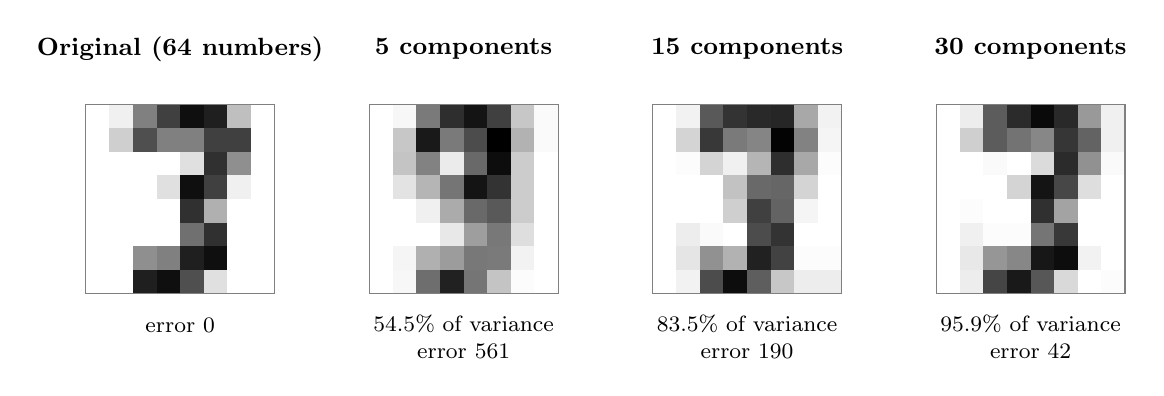
\begin{tikzpicture}
\node[font=\small\bfseries] at (1.2,3.1) {Original (64 numbers)};
\begin{scope}\fill[black!0] (0.00,2.10) rectangle ++(0.3,0.3);
\fill[black!6] (0.30,2.10) rectangle ++(0.3,0.3);
\fill[black!50] (0.60,2.10) rectangle ++(0.3,0.3);
\fill[black!75] (0.90,2.10) rectangle ++(0.3,0.3);
\fill[black!94] (1.20,2.10) rectangle ++(0.3,0.3);
\fill[black!88] (1.50,2.10) rectangle ++(0.3,0.3);
\fill[black!25] (1.80,2.10) rectangle ++(0.3,0.3);
\fill[black!0] (2.10,2.10) rectangle ++(0.3,0.3);
\fill[black!0] (0.00,1.80) rectangle ++(0.3,0.3);
\fill[black!19] (0.30,1.80) rectangle ++(0.3,0.3);
\fill[black!69] (0.60,1.80) rectangle ++(0.3,0.3);
\fill[black!50] (0.90,1.80) rectangle ++(0.3,0.3);
\fill[black!50] (1.20,1.80) rectangle ++(0.3,0.3);
\fill[black!75] (1.50,1.80) rectangle ++(0.3,0.3);
\fill[black!75] (1.80,1.80) rectangle ++(0.3,0.3);
\fill[black!0] (2.10,1.80) rectangle ++(0.3,0.3);
\fill[black!0] (0.00,1.50) rectangle ++(0.3,0.3);
\fill[black!0] (0.30,1.50) rectangle ++(0.3,0.3);
\fill[black!0] (0.60,1.50) rectangle ++(0.3,0.3);
\fill[black!0] (0.90,1.50) rectangle ++(0.3,0.3);
\fill[black!12] (1.20,1.50) rectangle ++(0.3,0.3);
\fill[black!81] (1.50,1.50) rectangle ++(0.3,0.3);
\fill[black!44] (1.80,1.50) rectangle ++(0.3,0.3);
\fill[black!0] (2.10,1.50) rectangle ++(0.3,0.3);
\fill[black!0] (0.00,1.20) rectangle ++(0.3,0.3);
\fill[black!0] (0.30,1.20) rectangle ++(0.3,0.3);
\fill[black!0] (0.60,1.20) rectangle ++(0.3,0.3);
\fill[black!12] (0.90,1.20) rectangle ++(0.3,0.3);
\fill[black!94] (1.20,1.20) rectangle ++(0.3,0.3);
\fill[black!75] (1.50,1.20) rectangle ++(0.3,0.3);
\fill[black!6] (1.80,1.20) rectangle ++(0.3,0.3);
\fill[black!0] (2.10,1.20) rectangle ++(0.3,0.3);
\fill[black!0] (0.00,0.90) rectangle ++(0.3,0.3);
\fill[black!0] (0.30,0.90) rectangle ++(0.3,0.3);
\fill[black!0] (0.60,0.90) rectangle ++(0.3,0.3);
\fill[black!0] (0.90,0.90) rectangle ++(0.3,0.3);
\fill[black!81] (1.20,0.90) rectangle ++(0.3,0.3);
\fill[black!31] (1.50,0.90) rectangle ++(0.3,0.3);
\fill[black!0] (1.80,0.90) rectangle ++(0.3,0.3);
\fill[black!0] (2.10,0.90) rectangle ++(0.3,0.3);
\fill[black!0] (0.00,0.60) rectangle ++(0.3,0.3);
\fill[black!0] (0.30,0.60) rectangle ++(0.3,0.3);
\fill[black!0] (0.60,0.60) rectangle ++(0.3,0.3);
\fill[black!0] (0.90,0.60) rectangle ++(0.3,0.3);
\fill[black!56] (1.20,0.60) rectangle ++(0.3,0.3);
\fill[black!81] (1.50,0.60) rectangle ++(0.3,0.3);
\fill[black!0] (1.80,0.60) rectangle ++(0.3,0.3);
\fill[black!0] (2.10,0.60) rectangle ++(0.3,0.3);
\fill[black!0] (0.00,0.30) rectangle ++(0.3,0.3);
\fill[black!0] (0.30,0.30) rectangle ++(0.3,0.3);
\fill[black!44] (0.60,0.30) rectangle ++(0.3,0.3);
\fill[black!50] (0.90,0.30) rectangle ++(0.3,0.3);
\fill[black!88] (1.20,0.30) rectangle ++(0.3,0.3);
\fill[black!94] (1.50,0.30) rectangle ++(0.3,0.3);
\fill[black!0] (1.80,0.30) rectangle ++(0.3,0.3);
\fill[black!0] (2.10,0.30) rectangle ++(0.3,0.3);
\fill[black!0] (0.00,0.00) rectangle ++(0.3,0.3);
\fill[black!0] (0.30,0.00) rectangle ++(0.3,0.3);
\fill[black!88] (0.60,0.00) rectangle ++(0.3,0.3);
\fill[black!94] (0.90,0.00) rectangle ++(0.3,0.3);
\fill[black!69] (1.20,0.00) rectangle ++(0.3,0.3);
\fill[black!12] (1.50,0.00) rectangle ++(0.3,0.3);
\fill[black!0] (1.80,0.00) rectangle ++(0.3,0.3);
\fill[black!0] (2.10,0.00) rectangle ++(0.3,0.3);
\draw[gray] (0,0) rectangle (2.4,2.4);
\end{scope}
\node[font=\footnotesize] at (1.2,-0.4) {error $0$};
\begin{scope}[xshift=3.6cm]
\node[font=\small\bfseries] at (1.2,3.1) {5 components};
\fill[black!0] (0.00,2.10) rectangle ++(0.3,0.3);
\fill[black!3] (0.30,2.10) rectangle ++(0.3,0.3);
\fill[black!52] (0.60,2.10) rectangle ++(0.3,0.3);
\fill[black!82] (0.90,2.10) rectangle ++(0.3,0.3);
\fill[black!92] (1.20,2.10) rectangle ++(0.3,0.3);
\fill[black!75] (1.50,2.10) rectangle ++(0.3,0.3);
\fill[black!22] (1.80,2.10) rectangle ++(0.3,0.3);
\fill[black!2] (2.10,2.10) rectangle ++(0.3,0.3);
\fill[black!0] (0.00,1.80) rectangle ++(0.3,0.3);
\fill[black!22] (0.30,1.80) rectangle ++(0.3,0.3);
\fill[black!90] (0.60,1.80) rectangle ++(0.3,0.3);
\fill[black!52] (0.90,1.80) rectangle ++(0.3,0.3);
\fill[black!70] (1.20,1.80) rectangle ++(0.3,0.3);
\fill[black!100] (1.50,1.80) rectangle ++(0.3,0.3);
\fill[black!30] (1.80,1.80) rectangle ++(0.3,0.3);
\fill[black!2] (2.10,1.80) rectangle ++(0.3,0.3);
\fill[black!0] (0.00,1.50) rectangle ++(0.3,0.3);
\fill[black!23] (0.30,1.50) rectangle ++(0.3,0.3);
\fill[black!49] (0.60,1.50) rectangle ++(0.3,0.3);
\fill[black!8] (0.90,1.50) rectangle ++(0.3,0.3);
\fill[black!59] (1.20,1.50) rectangle ++(0.3,0.3);
\fill[black!95] (1.50,1.50) rectangle ++(0.3,0.3);
\fill[black!20] (1.80,1.50) rectangle ++(0.3,0.3);
\fill[black!0] (2.10,1.50) rectangle ++(0.3,0.3);
\fill[black!0] (0.00,1.20) rectangle ++(0.3,0.3);
\fill[black!11] (0.30,1.20) rectangle ++(0.3,0.3);
\fill[black!29] (0.60,1.20) rectangle ++(0.3,0.3);
\fill[black!54] (0.90,1.20) rectangle ++(0.3,0.3);
\fill[black!92] (1.20,1.20) rectangle ++(0.3,0.3);
\fill[black!80] (1.50,1.20) rectangle ++(0.3,0.3);
\fill[black!20] (1.80,1.20) rectangle ++(0.3,0.3);
\fill[black!0] (2.10,1.20) rectangle ++(0.3,0.3);
\fill[black!0] (0.00,0.90) rectangle ++(0.3,0.3);
\fill[black!0] (0.30,0.90) rectangle ++(0.3,0.3);
\fill[black!6] (0.60,0.90) rectangle ++(0.3,0.3);
\fill[black!33] (0.90,0.90) rectangle ++(0.3,0.3);
\fill[black!59] (1.20,0.90) rectangle ++(0.3,0.3);
\fill[black!65] (1.50,0.90) rectangle ++(0.3,0.3);
\fill[black!20] (1.80,0.90) rectangle ++(0.3,0.3);
\fill[black!0] (2.10,0.90) rectangle ++(0.3,0.3);
\fill[black!0] (0.00,0.60) rectangle ++(0.3,0.3);
\fill[black!0] (0.30,0.60) rectangle ++(0.3,0.3);
\fill[black!0] (0.60,0.60) rectangle ++(0.3,0.3);
\fill[black!9] (0.90,0.60) rectangle ++(0.3,0.3);
\fill[black!38] (1.20,0.60) rectangle ++(0.3,0.3);
\fill[black!53] (1.50,0.60) rectangle ++(0.3,0.3);
\fill[black!13] (1.80,0.60) rectangle ++(0.3,0.3);
\fill[black!0] (2.10,0.60) rectangle ++(0.3,0.3);
\fill[black!0] (0.00,0.30) rectangle ++(0.3,0.3);
\fill[black!4] (0.30,0.30) rectangle ++(0.3,0.3);
\fill[black!31] (0.60,0.30) rectangle ++(0.3,0.3);
\fill[black!39] (0.90,0.30) rectangle ++(0.3,0.3);
\fill[black!53] (1.20,0.30) rectangle ++(0.3,0.3);
\fill[black!52] (1.50,0.30) rectangle ++(0.3,0.3);
\fill[black!5] (1.80,0.30) rectangle ++(0.3,0.3);
\fill[black!0] (2.10,0.30) rectangle ++(0.3,0.3);
\fill[black!0] (0.00,0.00) rectangle ++(0.3,0.3);
\fill[black!3] (0.30,0.00) rectangle ++(0.3,0.3);
\fill[black!57] (0.60,0.00) rectangle ++(0.3,0.3);
\fill[black!87] (0.90,0.00) rectangle ++(0.3,0.3);
\fill[black!54] (1.20,0.00) rectangle ++(0.3,0.3);
\fill[black!23] (1.50,0.00) rectangle ++(0.3,0.3);
\fill[black!1] (1.80,0.00) rectangle ++(0.3,0.3);
\fill[black!0] (2.10,0.00) rectangle ++(0.3,0.3);
\draw[gray] (0,0) rectangle (2.4,2.4);

\node[font=\footnotesize,align=center] at (1.2,-0.55) {54.5\% of variance\\error $561$};
\end{scope}
\begin{scope}[xshift=7.2cm]
\node[font=\small\bfseries] at (1.2,3.1) {15 components};
\fill[black!0] (0.00,2.10) rectangle ++(0.3,0.3);
\fill[black!5] (0.30,2.10) rectangle ++(0.3,0.3);
\fill[black!65] (0.60,2.10) rectangle ++(0.3,0.3);
\fill[black!80] (0.90,2.10) rectangle ++(0.3,0.3);
\fill[black!84] (1.20,2.10) rectangle ++(0.3,0.3);
\fill[black!85] (1.50,2.10) rectangle ++(0.3,0.3);
\fill[black!34] (1.80,2.10) rectangle ++(0.3,0.3);
\fill[black!5] (2.10,2.10) rectangle ++(0.3,0.3);
\fill[black!0] (0.00,1.80) rectangle ++(0.3,0.3);
\fill[black!17] (0.30,1.80) rectangle ++(0.3,0.3);
\fill[black!78] (0.60,1.80) rectangle ++(0.3,0.3);
\fill[black!52] (0.90,1.80) rectangle ++(0.3,0.3);
\fill[black!48] (1.20,1.80) rectangle ++(0.3,0.3);
\fill[black!99] (1.50,1.80) rectangle ++(0.3,0.3);
\fill[black!49] (1.80,1.80) rectangle ++(0.3,0.3);
\fill[black!4] (2.10,1.80) rectangle ++(0.3,0.3);
\fill[black!0] (0.00,1.50) rectangle ++(0.3,0.3);
\fill[black!1] (0.30,1.50) rectangle ++(0.3,0.3);
\fill[black!17] (0.60,1.50) rectangle ++(0.3,0.3);
\fill[black!6] (0.90,1.50) rectangle ++(0.3,0.3);
\fill[black!29] (1.20,1.50) rectangle ++(0.3,0.3);
\fill[black!82] (1.50,1.50) rectangle ++(0.3,0.3);
\fill[black!34] (1.80,1.50) rectangle ++(0.3,0.3);
\fill[black!1] (2.10,1.50) rectangle ++(0.3,0.3);
\fill[black!0] (0.00,1.20) rectangle ++(0.3,0.3);
\fill[black!0] (0.30,1.20) rectangle ++(0.3,0.3);
\fill[black!0] (0.60,1.20) rectangle ++(0.3,0.3);
\fill[black!24] (0.90,1.20) rectangle ++(0.3,0.3);
\fill[black!59] (1.20,1.20) rectangle ++(0.3,0.3);
\fill[black!60] (1.50,1.20) rectangle ++(0.3,0.3);
\fill[black!17] (1.80,1.20) rectangle ++(0.3,0.3);
\fill[black!0] (2.10,1.20) rectangle ++(0.3,0.3);
\fill[black!0] (0.00,0.90) rectangle ++(0.3,0.3);
\fill[black!0] (0.30,0.90) rectangle ++(0.3,0.3);
\fill[black!0] (0.60,0.90) rectangle ++(0.3,0.3);
\fill[black!19] (0.90,0.90) rectangle ++(0.3,0.3);
\fill[black!75] (1.20,0.90) rectangle ++(0.3,0.3);
\fill[black!61] (1.50,0.90) rectangle ++(0.3,0.3);
\fill[black!4] (1.80,0.90) rectangle ++(0.3,0.3);
\fill[black!0] (2.10,0.90) rectangle ++(0.3,0.3);
\fill[black!0] (0.00,0.60) rectangle ++(0.3,0.3);
\fill[black!7] (0.30,0.60) rectangle ++(0.3,0.3);
\fill[black!2] (0.60,0.60) rectangle ++(0.3,0.3);
\fill[black!0] (0.90,0.60) rectangle ++(0.3,0.3);
\fill[black!70] (1.20,0.60) rectangle ++(0.3,0.3);
\fill[black!80] (1.50,0.60) rectangle ++(0.3,0.3);
\fill[black!0] (1.80,0.60) rectangle ++(0.3,0.3);
\fill[black!0] (2.10,0.60) rectangle ++(0.3,0.3);
\fill[black!0] (0.00,0.30) rectangle ++(0.3,0.3);
\fill[black!10] (0.30,0.30) rectangle ++(0.3,0.3);
\fill[black!43] (0.60,0.30) rectangle ++(0.3,0.3);
\fill[black!30] (0.90,0.30) rectangle ++(0.3,0.3);
\fill[black!87] (1.20,0.30) rectangle ++(0.3,0.3);
\fill[black!74] (1.50,0.30) rectangle ++(0.3,0.3);
\fill[black!1] (1.80,0.30) rectangle ++(0.3,0.3);
\fill[black!1] (2.10,0.30) rectangle ++(0.3,0.3);
\fill[black!0] (0.00,0.00) rectangle ++(0.3,0.3);
\fill[black!5] (0.30,0.00) rectangle ++(0.3,0.3);
\fill[black!70] (0.60,0.00) rectangle ++(0.3,0.3);
\fill[black!95] (0.90,0.00) rectangle ++(0.3,0.3);
\fill[black!63] (1.20,0.00) rectangle ++(0.3,0.3);
\fill[black!22] (1.50,0.00) rectangle ++(0.3,0.3);
\fill[black!7] (1.80,0.00) rectangle ++(0.3,0.3);
\fill[black!7] (2.10,0.00) rectangle ++(0.3,0.3);
\draw[gray] (0,0) rectangle (2.4,2.4);

\node[font=\footnotesize,align=center] at (1.2,-0.55) {83.5\% of variance\\error $190$};
\end{scope}
\begin{scope}[xshift=10.8cm]
\node[font=\small\bfseries] at (1.2,3.1) {30 components};
\fill[black!0] (0.00,2.10) rectangle ++(0.3,0.3);
\fill[black!7] (0.30,2.10) rectangle ++(0.3,0.3);
\fill[black!64] (0.60,2.10) rectangle ++(0.3,0.3);
\fill[black!83] (0.90,2.10) rectangle ++(0.3,0.3);
\fill[black!96] (1.20,2.10) rectangle ++(0.3,0.3);
\fill[black!84] (1.50,2.10) rectangle ++(0.3,0.3);
\fill[black!40] (1.80,2.10) rectangle ++(0.3,0.3);
\fill[black!6] (2.10,2.10) rectangle ++(0.3,0.3);
\fill[black!0] (0.00,1.80) rectangle ++(0.3,0.3);
\fill[black!19] (0.30,1.80) rectangle ++(0.3,0.3);
\fill[black!64] (0.60,1.80) rectangle ++(0.3,0.3);
\fill[black!55] (0.90,1.80) rectangle ++(0.3,0.3);
\fill[black!47] (1.20,1.80) rectangle ++(0.3,0.3);
\fill[black!79] (1.50,1.80) rectangle ++(0.3,0.3);
\fill[black!61] (1.80,1.80) rectangle ++(0.3,0.3);
\fill[black!6] (2.10,1.80) rectangle ++(0.3,0.3);
\fill[black!0] (0.00,1.50) rectangle ++(0.3,0.3);
\fill[black!0] (0.30,1.50) rectangle ++(0.3,0.3);
\fill[black!2] (0.60,1.50) rectangle ++(0.3,0.3);
\fill[black!0] (0.90,1.50) rectangle ++(0.3,0.3);
\fill[black!14] (1.20,1.50) rectangle ++(0.3,0.3);
\fill[black!83] (1.50,1.50) rectangle ++(0.3,0.3);
\fill[black!43] (1.80,1.50) rectangle ++(0.3,0.3);
\fill[black!2] (2.10,1.50) rectangle ++(0.3,0.3);
\fill[black!0] (0.00,1.20) rectangle ++(0.3,0.3);
\fill[black!0] (0.30,1.20) rectangle ++(0.3,0.3);
\fill[black!0] (0.60,1.20) rectangle ++(0.3,0.3);
\fill[black!17] (0.90,1.20) rectangle ++(0.3,0.3);
\fill[black!92] (1.20,1.20) rectangle ++(0.3,0.3);
\fill[black!72] (1.50,1.20) rectangle ++(0.3,0.3);
\fill[black!13] (1.80,1.20) rectangle ++(0.3,0.3);
\fill[black!0] (2.10,1.20) rectangle ++(0.3,0.3);
\fill[black!0] (0.00,0.90) rectangle ++(0.3,0.3);
\fill[black!1] (0.30,0.90) rectangle ++(0.3,0.3);
\fill[black!0] (0.60,0.90) rectangle ++(0.3,0.3);
\fill[black!0] (0.90,0.90) rectangle ++(0.3,0.3);
\fill[black!81] (1.20,0.90) rectangle ++(0.3,0.3);
\fill[black!36] (1.50,0.90) rectangle ++(0.3,0.3);
\fill[black!0] (1.80,0.90) rectangle ++(0.3,0.3);
\fill[black!0] (2.10,0.90) rectangle ++(0.3,0.3);
\fill[black!0] (0.00,0.60) rectangle ++(0.3,0.3);
\fill[black!6] (0.30,0.60) rectangle ++(0.3,0.3);
\fill[black!1] (0.60,0.60) rectangle ++(0.3,0.3);
\fill[black!1] (0.90,0.60) rectangle ++(0.3,0.3);
\fill[black!54] (1.20,0.60) rectangle ++(0.3,0.3);
\fill[black!78] (1.50,0.60) rectangle ++(0.3,0.3);
\fill[black!0] (1.80,0.60) rectangle ++(0.3,0.3);
\fill[black!0] (2.10,0.60) rectangle ++(0.3,0.3);
\fill[black!0] (0.00,0.30) rectangle ++(0.3,0.3);
\fill[black!9] (0.30,0.30) rectangle ++(0.3,0.3);
\fill[black!41] (0.60,0.30) rectangle ++(0.3,0.3);
\fill[black!47] (0.90,0.30) rectangle ++(0.3,0.3);
\fill[black!91] (1.20,0.30) rectangle ++(0.3,0.3);
\fill[black!95] (1.50,0.30) rectangle ++(0.3,0.3);
\fill[black!5] (1.80,0.30) rectangle ++(0.3,0.3);
\fill[black!0] (2.10,0.30) rectangle ++(0.3,0.3);
\fill[black!0] (0.00,0.00) rectangle ++(0.3,0.3);
\fill[black!7] (0.30,0.00) rectangle ++(0.3,0.3);
\fill[black!73] (0.60,0.00) rectangle ++(0.3,0.3);
\fill[black!90] (0.90,0.00) rectangle ++(0.3,0.3);
\fill[black!66] (1.20,0.00) rectangle ++(0.3,0.3);
\fill[black!15] (1.50,0.00) rectangle ++(0.3,0.3);
\fill[black!0] (1.80,0.00) rectangle ++(0.3,0.3);
\fill[black!1] (2.10,0.00) rectangle ++(0.3,0.3);
\draw[gray] (0,0) rectangle (2.4,2.4);

\node[font=\footnotesize,align=center] at (1.2,-0.55) {95.9\% of variance\\error $42$};
\end{scope}
\end{tikzpicture}}
\caption{One handwritten digit reconstructed from 5, 15 and 30 principal components (real data; error = sum of squared pixel errors).}\label{fig:digitrec}
\end{figure}

\begin{explain}
The first picture is the original $8\times8$ image (dark = more ink). With only \textbf{5 components} we get a blurry blob: the rough position of the ink is right but details are missing (squared error $561$). With \textbf{15 components} the shape of the ``3'' emerges (error $190$), and with \textbf{30 components} the digit is almost identical to the original (error $42$, against $1149$ for describing it by the average digit alone). Each extra component adds detail; the first few capture the coarse shape.
\end{explain}

Now we use PCA as \emph{preprocessing} for a classifier. We trained logistic regression on the PCA-reduced digits (1347 training and 450 test images):

\begin{center}
\begin{tabular}{@{}rcccc@{}}
\toprule
\textbf{Components} & 2 & 5 & 10 & 20\\
Test accuracy & 0.636 & 0.867 & 0.922 & 0.951\\
Reconstruction MSE (per pixel) & 13.31 & 8.56 & 4.96 & 2.07\\
\midrule
\textbf{Components} & 29 & 40 & 64 (all) & \\
Test accuracy & 0.967 & \textbf{0.976} & 0.973 & \\
Reconstruction MSE & 0.90 & 0.24 & 0 & \\
\bottomrule
\end{tabular}
\end{center}

\noindent \textbf{Read the table:} with only \textbf{29} of 64 features (a 55\% reduction) accuracy is $0.967$, close to the full $0.973$, and with \textbf{40} components it is $0.976$, slightly \emph{better} than with all features: the discarded components were mostly noise. Using PCA(0.95), the library keeps the smallest number of components explaining $95\%$ of the variance (here $28$ on the training data).

\subsection{Real Example 3: Why You Must Scale the Features}

PCA looks for directions of maximum \emph{variance}, so a feature with large numbers will dominate. The wine dataset has $13$ chemical measurements; one of them, proline, has values in the hundreds or thousands while the others are around $0$--$10$.

\begin{figure}[!htbp]
\centering
\begin{tikzpicture}
\begin{axis}[ybar,width=11cm,height=6cm,bar width=14pt,ylabel={explained variance ratio},symbolic x coords={PC1,PC2,PC3},xtick=data,ymin=0,ymax=1.2,
  point meta=y,nodes near coords={\pgfmathprintnumber[fixed,precision=3]{\pgfplotspointmeta}},every node near coord/.append style={font=\scriptsize},legend style={at={(0.98,0.97)},anchor=north east,font=\small},ymajorgrids,grid style={gray!18},enlarge x limits=0.3]
\addplot[fill=mlred!60,draw=mlred] coordinates {(PC1,0.998)(PC2,0.002)(PC3,0.000)};
\addplot[fill=mlgreen!60,draw=mlgreen] coordinates {(PC1,0.362)(PC2,0.192)(PC3,0.111)};
\legend{raw features,standardised features}
\end{axis}
\end{tikzpicture}
\caption{PCA on the wine data with and without standardising the features (real results).}\label{fig:winescale}
\end{figure}

\begin{explain}
\textbf{Red bars (raw data):} the first component alone claims $99.8\%$ of the variance and the others are almost $0$. This is an \emph{artefact of units}: the loading of proline on PC1 is $1.00$ and all other features have loadings near $0$, so PC1 is simply ``the proline column''. \textbf{Green bars (standardised data):} after scaling every feature to mean $0$ and standard deviation $1$, the variance is shared among several components ($36.2\%$, $19.2\%$, $11.1\%$): the 13 features all contribute. Without scaling, the PCA would have thrown away all the other chemistry.
\end{explain}

\begin{warning}
\textbf{Always standardise the features before PCA} when they have different units or ranges (for example height in metres and weight in grams). Only skip scaling when all features are measured in the same units (e.g.\ pixel intensities).
\end{warning}

\subsection{Properties, Limits and Variants}

\paragraph{Properties.}
\begin{itemize}
  \item The principal components are \textbf{orthogonal}, and the new coordinates $z_1,z_2,\dots$ are \textbf{uncorrelated}.
  \item The total variance is preserved: $\sum\lambda_j=\text{trace}(\mathbf C)$.
  \item PCA is \textbf{sensitive to outliers} and to the \textbf{scale} of the features.
\end{itemize}

\paragraph{Limits.}
\begin{itemize}
  \item \textbf{Linear only:} it cannot unroll curved data (Swiss roll result above).
  \item \textbf{High variance $\neq$ useful:} PCA ignores labels; a direction with small variance may be exactly the one that separates the classes (then LDA is better).
  \item Components are combinations of all features and may be hard to interpret.
\end{itemize}

\paragraph{Variants.}

\begin{definition}[: Randomised, Incremental and Kernel PCA]
\begin{itemize}
  \item \textbf{Randomised PCA:} uses a stochastic algorithm that quickly approximates the first $m$ components; much faster when $m\ll d$.
  \item \textbf{Incremental PCA:} processes the data in mini-batches, so it works when the dataset does not fit in memory or arrives as a stream (online learning).
  \item \textbf{Kernel PCA:} applies PCA \emph{after} an implicit non-linear mapping, using the \emph{kernel trick} of Chapter~6 (the RBF kernel $e^{-\gamma\|\vect a-\vect b\|^2}$, for example). It can find non-linear structure.
\end{itemize}
\end{definition}

\begin{example}[: Kernel PCA on two concentric circles]
Two concentric circles (300 points) cannot be separated by a line. We reduced them to 2-D with PCA and with RBF Kernel PCA ($\gamma=10$), then trained logistic regression:

\begin{center}
\begin{tabular}{@{}lc@{}}
\toprule
\textbf{Representation} & \textbf{Logistic-regression accuracy}\\
\midrule
Raw 2-D coordinates & 0.51\\
Linear PCA (2 components) & 0.51\\
RBF Kernel PCA (2 components) & \textbf{1.00}\\
\bottomrule
\end{tabular}
\end{center}
Linear PCA only rotates the circles, so a straight line still cannot separate them. Kernel PCA ``unfolds'' them so that the two rings become linearly separable. (The kernel parameter $\gamma$ must be tuned, just as for SVMs.)
\end{example}

\begin{tryit}
\begin{lstlisting}
from sklearn.datasets import load_digits
from sklearn.decomposition import PCA
from sklearn.linear_model import LogisticRegression
from sklearn.model_selection import train_test_split
import numpy as np

X, y = load_digits(return_X_y=True)
Xtr, Xte, ytr, yte = train_test_split(X, y, test_size=0.25,
                                      random_state=42)

pca = PCA().fit(X)
cum = np.cumsum(pca.explained_variance_ratio_)
print(np.searchsorted(cum, 0.95) + 1)       # 29 components

for k in [2, 10, 29, 40]:
    p = PCA(n_components=k).fit(Xtr)
    clf = LogisticRegression(max_iter=3000).fit(p.transform(Xtr), ytr)
    print(k, round(clf.score(p.transform(Xte), yte), 3))
# 2 -> 0.636, 10 -> 0.922, 29 -> 0.967, 40 -> 0.976

# keep enough components for 95% of the variance
print(PCA(n_components=0.95).fit(Xtr).n_components_)   # 28
\end{lstlisting}
\emph{Challenge:} apply \texttt{PCA(2)} to the iris data (with and without \texttt{StandardScaler}) and compare the explained variance ratios with the table above.
\end{tryit}

\procon{Principal Component Analysis}
{\item Fast and simple; solved exactly by an eigen-decomposition
 \item Removes redundancy and noise; produces uncorrelated features
 \item Fewer features: faster and less overfitting
 \item Enables 2-D/3-D visualisation and compression}
{\item Only captures \emph{linear} structure
 \item Must scale features first; sensitive to outliers
 \item High variance does not always mean high usefulness (ignores labels)
 \item Components are hard to interpret}
{\item Image compression and eigenfaces
 \item Preprocessing for classifiers and clustering
 \item Visualising high-dimensional data
 \item Noise reduction; finance and genetics}

\procon{Kernel PCA}
{\item Captures non-linear structure
 \item Can unfold circles and curved clusters
 \item Same easy interface as PCA
 \item Uses the familiar kernel trick}
{\item Needs the kernel and its parameters to be tuned
 \item Memory and time grow with the square of the number of points
 \item Reconstruction (pre-image) is difficult
 \item Components are even harder to interpret}
{\item Pre-processing for classifiers on curved data
 \item Non-linear visualisation and denoising
 \item Pattern recognition tasks}

%====================================================================
\section{Choosing a Dimensionality-Reduction Method}

\begin{center}
\small
\begin{tabular}{@{}p{3cm}p{3.7cm}p{3.7cm}p{3.5cm}@{}}
\toprule
 & \textbf{PCA} & \textbf{Kernel PCA / Isomap / LLE} & \textbf{t-SNE}\\
\midrule
Type & Linear projection & Non-linear & Non-linear (visualisation)\\
Keeps & Global variance & Non-linear structure & Local neighbourhoods\\
New data? & Yes (\texttt{transform}) & Yes (kernel PCA) / limited & \textbf{No}\\
Speed & \textbf{Very fast} & Slower & Slow\\
Inverse (reconstruction) & Yes & Hard & No\\
Typical output & 2 to hundreds of dimensions & few dimensions & 2-D or 3-D picture\\
Use for & Preprocessing, compression & Curved data & Looking at clusters\\
\bottomrule
\end{tabular}
\end{center}

\begin{figure}[!htbp]
\centering
\resizebox{\linewidth}{!}{%
\begin{tikzpicture}[q/.style={draw,rounded corners,thick,fill=mlblue!10,draw=mlblue,align=center,font=\small,inner sep=6pt,text width=4.2cm},
 a/.style={draw,rounded corners,very thick,align=center,font=\small\bfseries,inner sep=6pt,text width=3.0cm},arr/.style={-{Stealth},thick}]
\node[q] (q1) at (0,0) {Is the goal only to \emph{look at} the data in 2-D?};
\node[a,fill=mlorange!18,draw=mlorange] (ts) at (6.2,1.4) {t-SNE (or PCA to 2-D first)};
\node[q] (q2) at (0,-3) {Is the structure curved (non-linear)?};
\node[a,fill=mlpurple!14,draw=mlpurple] (kp) at (6.2,-1.5) {Kernel PCA, Isomap or LLE};
\node[a,fill=mlgreen!18,draw=mlgreen] (pc) at (6.2,-4.4) {PCA (standardise first!)};
\draw[arr] (q1)--(ts) node[midway,above,font=\footnotesize]{yes};
\draw[arr] (q1)--(q2) node[midway,left,font=\footnotesize]{no};
\draw[arr] (q2)--(kp) node[midway,above,font=\footnotesize]{yes};
\draw[arr] (q2)--(pc) node[pos=0.45,below left,font=\footnotesize]{no};
\pic[scale=1.2] at (10.6,-1.8) {smile};
\bubble[text width=3.6cm]{12.5,-3.8}{10.7,-2.2}{PCA is the first thing to try!}
\end{tikzpicture}}
\caption{A simple guide for choosing a dimensionality-reduction method.}\label{fig:choosedr}
\end{figure}

\begin{explain}
Start from the top question. If you only want to \emph{draw} the data, use t-SNE (often after reducing to about 50 dimensions with PCA) or simply PCA with two components. If you need the reduced features for \emph{learning}, ask whether the data lie on a curved surface: if yes, try a non-linear method such as Kernel PCA, Isomap or LLE; if not, use ordinary PCA, which is fast, invertible and applicable to new data. Remember to standardise the features before PCA.
\end{explain}

%====================================================================
\begin{summary}
\begin{itemize}
  \item \textbf{Dimensionality reduction} maps $d$ features to $m<d$ while keeping the useful information (unsupervised).
  \item \textbf{Curse of dimensionality:} space grows exponentially, so data become sparse ($10^d$ cells), almost all points lie near the boundary ($1-0.998^d$), distances concentrate (contrast $40.7\to0.13$ from 2-D to 1000-D) and algorithms such as k-NN degrade ($94.8\%\to37.1\%$ with junk features).
  \item \textbf{Projection} (linear: PCA, random projection, LDA) vs.\ \textbf{manifold learning} (non-linear: Isomap, LLE, t-SNE, kernel PCA); the manifold hypothesis says real data lie near a low-dimensional manifold.
  \item \textbf{PCA:} centre (and scale) the data, covariance matrix $\mathbf C$, eigenvalues $\lambda_j$ (variances) and eigenvectors (components), project $\mathbf Z=\tilde{\mathbf X}\mathbf W_m$. Explained variance ratio $\lambda_j/\sum\lambda_i$; keep components for $95\%$; reconstruction error $=$ discarded eigenvalues.
  \item Worked example: $\mathbf C=\begin{bmatrix}2.5&2\\2&2.5\end{bmatrix}$, $\lambda=4.5,0.5$, PC1 $=(1,1)/\sqrt2$ explains $90\%$.
  \item \textbf{Scale first:} on the wine data raw PCA gives $99.8\%$ on PC1 (an artefact of units).
  \item \textbf{Variants:} Randomised, Incremental and Kernel PCA (accuracy $0.51\to1.00$ on circles).
\end{itemize}
\end{summary}

%====================================================================
\section*{Exam Corner}
\addcontentsline{toc}{section}{Exam Corner}

\subsection*{A.\ Very Short Answer Questions (2 marks each)}
\begin{enumerate}
  \item Define dimensionality reduction. Give two reasons for using it. \qmarks{2}
  \item What is the curse of dimensionality? \qmarks{2}
  \item Why do distances lose meaning in high dimensions? \qmarks{2}
  \item Differentiate between projection and manifold learning. \qmarks{2}
  \item What is the manifold hypothesis? \qmarks{2}
  \item Name two linear and two non-linear dimensionality-reduction methods. \qmarks{2}
  \item Define principal component analysis. \qmarks{2}
  \item What is the explained variance ratio? \qmarks{2}
  \item What is the relation between eigenvalues of the covariance matrix and the variance along principal components? \qmarks{2}
  \item Why must features be standardised before PCA? \qmarks{2}
  \item How can the number of principal components be chosen? \qmarks{2}
  \item What is Kernel PCA? When is it useful? \qmarks{2}
\end{enumerate}

\begin{modelans}[: Q2, Q5 and Q10]
\textbf{Q2.} The curse of dimensionality is the set of problems that arise when the number of features is large: the space grows exponentially so data become sparse, distances between points become almost equal, most points lie near the boundary, and the amount of data required grows exponentially, so learning algorithms (especially distance-based ones) overfit or lose accuracy.\par
\textbf{Q5.} The manifold hypothesis states that real-world high-dimensional data (images, speech, \dots) lie close to a lower-dimensional manifold embedded in the high-dimensional space, because only a few hidden factors vary.\par
\textbf{Q10.} PCA maximises variance, so a feature with a large numeric range dominates the first components regardless of its importance (e.g.\ on the wine data an unscaled PCA gives $99.8\%$ of the variance to one feature). Standardising puts all features on the same scale.
\end{modelans}

\subsection*{B.\ Short Answer Questions (5 marks each)}
\begin{enumerate}
  \item Explain the curse of dimensionality with examples. \qmarks{5}
  \item Explain how high dimensionality affects k-NN and other distance-based algorithms. \qmarks{5}
  \item Explain the two main approaches to dimensionality reduction with a diagram. \qmarks{5}
  \item Explain Isomap, LLE and t-SNE briefly. \qmarks{5}
  \item Explain the PCA algorithm step by step. \qmarks{5}
  \item Derive why principal components are eigenvectors of the covariance matrix. \qmarks{5}
  \item Explain how to choose the number of principal components (scree plot and cumulative variance). \qmarks{5}
  \item Explain PCA for compression with reconstruction error. \qmarks{5}
  \item Explain Randomised PCA, Incremental PCA and Kernel PCA. \qmarks{5}
  \item List the advantages and disadvantages of PCA. \qmarks{5}
\end{enumerate}

\begin{modelans}[: B5 (outline for 5 marks)]
(1)~Standardise or centre the data. (2)~Compute the covariance matrix $\mathbf C=\frac1{n-1}\tilde{\mathbf X}^{\!\top}\tilde{\mathbf X}$. (3)~Compute its eigenvalues $\lambda_j$ and unit eigenvectors $\vect w_j$. (4)~Sort the eigenvectors by decreasing eigenvalue (these are the principal components) and choose the number $m$ to keep using the explained variance ratio $\lambda_j/\sum\lambda_i$. (5)~Project: $\mathbf Z=\tilde{\mathbf X}\mathbf W_m$. (6)~Optionally reconstruct $\hat{\mathbf X}=\mathbf Z\mathbf W_m^{\!\top}+\text{mean}$; the error equals the sum of the discarded eigenvalues. Add a small 2-D example and a diagram of the principal axes.
\end{modelans}

\subsection*{C.\ Long Answer Questions (10 marks each)}
\begin{enumerate}
  \item Explain the curse of dimensionality in detail. Discuss its effects on volume, distances, data requirements and learning algorithms, and suggest remedies. \qmarks{10}
  \item Explain projection and manifold learning. Describe PCA, Isomap, LLE and t-SNE, and compare them. \qmarks{10}
  \item Explain PCA with the full algorithm and perform it by hand on a small two-dimensional dataset: covariance matrix, eigenvalues, eigenvectors, projection and explained variance. \qmarks{10}
  \item Explain how the number of components is chosen in PCA and discuss the importance of feature scaling. Explain how PCA is used for compression, visualisation and preprocessing. \qmarks{10}
  \item Describe the variants of PCA (Randomised, Incremental and Kernel PCA) and explain when each is used. \qmarks{10}
  \item Discuss the advantages, disadvantages and limitations of PCA and compare it with non-linear dimensionality-reduction methods. \qmarks{10}
\end{enumerate}

\begin{modelans}[: C3 (a second numerical solution)]
Data $(1,2),(3,4),(5,6)$. Means $(3,4)$; centred points $(-2,-2),(0,0),(2,2)$. Covariance ($n-1=2$): $s_{xx}=\frac{4+0+4}{2}=4$, $s_{yy}=4$, $s_{xy}=4$; $\mathbf C=\begin{bmatrix}4&4\\4&4\end{bmatrix}$.\par
$\det(\mathbf C-\lambda\mathbf I)=(4-\lambda)^2-16=0\Rightarrow\lambda_1=8,\ \lambda_2=0$. $\vect w_1=\frac1{\sqrt2}(1,1)$. Explained variance of PC1 $=8/8=100\%$.\par
Projections $z_1=\frac{(x-3)+(y-4)}{\sqrt2}=(-2.828,\ 0,\ 2.828)$. The points lie exactly on a line, so one component describes them \emph{without any loss}.
\end{modelans}

\subsection*{D.\ Numerical Problems}
\begin{enumerate}
  \item The eigenvalues of a covariance matrix are $6,\ 3,\ 1$. Find the explained variance ratios and the number of components needed for at least $85\%$ of the variance. \textit{(Answer: $0.6,0.3,0.1$; two components give $90\%\ge85\%$.)}
  \item Find the eigenvalues and eigenvectors of $\mathbf C=\begin{bmatrix}3&1\\1&3\end{bmatrix}$ and the explained variance of PC1. \textit{(Answer: $(3-\lambda)^2=1\Rightarrow\lambda=4,2$; $\vect w_1=(1,1)/\sqrt2$, $\vect w_2=(1,-1)/\sqrt2$; PC1 explains $4/6=66.7\%$.)}
  \item Perform PCA on $(1,2),(3,4),(5,6)$ and find the explained variance of PC1. \textit{(Answer: $\mathbf C=\begin{bmatrix}4&4\\4&4\end{bmatrix}$, $\lambda=8,0$; $100\%$.)}
  \item The mean is $(1,1)$ and the first component is $\vect w_1=(0.6,0.8)$. Project $(4,3)$ and reconstruct it. \textit{(Answer: centred $(3,2)$; $z=3(0.6)+2(0.8)=3.4$; $\hat{\vect x}=(1,1)+3.4(0.6,0.8)=(3.04,3.72)$.)}
  \item A point is uniformly distributed in the hypercube $[0,1]^{50}$. Find the probability that it lies within $0.001$ of a border. \textit{(Answer: $1-0.998^{50}=1-0.905=0.095$.)}
  \item With 5 intervals per feature, how many cells are there for $d=8$ features? \textit{(Answer: $5^8=390\,625$.)}
  \item What fraction of the unit square is covered by a disc of radius $0.1$ (ignoring edge effects)? \textit{(Answer: $\pi(0.1)^2=0.0314$, i.e.\ $3.1\%$.)}
  \item A covariance matrix has total variance $10$; the first eigenvalue is $8$. How much variance is lost if only PC1 is kept? \textit{(Answer: $2$, i.e.\ $20\%$.)}
  \item Digit images have 64 features; PCA keeps 29 components. What fraction of the numbers is stored and what is the reduction? \textit{(Answer: $29/64=45\%$; $64/29=2.2\times$ smaller.)}
  \item Singular values of a centred matrix with $n=5$ rows are $s_1=4.243$ and $s_2=1.414$. Find the eigenvalues and the explained variance of PC1. \textit{(Answer: $\lambda=s^2/(n-1)=4.5,\ 0.5$; $90\%$.)}
\end{enumerate}

\subsection*{E.\ Multiple-Choice Questions}
\begin{enumerate}
  \item In high dimensions the relative contrast between the nearest and farthest neighbour: \\
  (a) increases \quad (b) decreases \quad (c) stays the same \quad (d) becomes infinite
  \item Which method is a \emph{non-linear} dimensionality reduction? \\
  (a) PCA \quad (b) Random projection \quad (c) Isomap \quad (d) LDA with linear kernel
  \item The first principal component is the direction of: \\
  (a) minimum variance \quad (b) maximum variance \quad (c) maximum mean \quad (d) minimum distance
  \item Principal components are: \\
  (a) parallel \quad (b) orthogonal \quad (c) identical \quad (d) random
  \item The variance along a principal component equals: \\
  (a) the eigenvalue \quad (b) the eigenvector \quad (c) the mean \quad (d) the trace
  \item PCA is computed from the eigen-decomposition of the: \\
  (a) confusion matrix \quad (b) covariance matrix \quad (c) distance matrix \quad (d) weight matrix
  \item If eigenvalues are $4,2,2,2$ the explained variance ratio of PC1 is: \\
  (a) 0.25 \quad (b) 0.4 \quad (c) 0.5 \quad (d) 0.8
  \item Before PCA with features in different units we should: \\
  (a) do nothing \quad (b) standardise the features \quad (c) add noise \quad (d) remove labels
  \item Which PCA variant handles data that do not fit in memory? \\
  (a) Kernel PCA \quad (b) Incremental PCA \quad (c) Sparse PCA \quad (d) none
  \item Kernel PCA is used to capture: \\
  (a) linear structure only \quad (b) non-linear structure \quad (c) labels \quad (d) outliers
  \item The reconstruction error of PCA with $m$ components equals: \\
  (a) the sum of the first $m$ eigenvalues \quad (b) the sum of the discarded eigenvalues \quad (c) zero \quad (d) the largest eigenvalue
  \item t-SNE is mainly used for: \\
  (a) compression \quad (b) visualisation \quad (c) regression \quad (d) scaling
\end{enumerate}
\textbf{Answers:} 1-b,\ 2-c,\ 3-b,\ 4-b,\ 5-a,\ 6-b,\ 7-b,\ 8-b,\ 9-b,\ 10-b,\ 11-b,\ 12-b.

\subsection*{F.\ Practice Problems}
\begin{enumerate}
  \item For the data $(2,0),(0,2),(-2,0),(0,-2)$ find the covariance matrix and eigenvalues. What does the result say about PCA on this data? \textit{(Answer: $\mathbf C=\begin{bmatrix}8/3&0\\0&8/3\end{bmatrix}$; equal eigenvalues, so no direction is preferred: PCA cannot reduce this data.)}
  \item Using the five-point example, compute $z_1$ for a new point $(6,6)$ and its reconstruction. \textit{(Answer: centred $(3,3)$; $z_1=\frac{6}{\sqrt2}=4.243$; reconstruction $(6,6)$, exactly on PC1.)}
  \item \textbf{Coding:} apply PCA to the \emph{wine} data with and without \texttt{StandardScaler} and plot the first two components, coloured by wine type.
  \item \textbf{Coding:} use \texttt{PCA(n\_components=0.95)} to compress the \emph{digits} data and measure the accuracy of k-NN before and after.
  \item \textbf{Coding:} use \texttt{sklearn.manifold.TSNE} to draw the digits in 2-D, coloured by digit.
  \item Draw a labelled diagram of PCA on a two-dimensional elongated cloud with both principal axes.
\end{enumerate}

\begin{revision}
\begin{center}\small
\begin{tabular}{@{}p{3.6cm}p{9.6cm}@{}}
\toprule
\textbf{Topic} & \textbf{One-line recall}\\
\midrule
Dimensionality reduction & $d\to m<d$ keeping useful information; unsupervised.\\
Curse of dimensionality & Sparse data ($10^d$ cells), points near border ($1-0.998^d$), distances concentrate, k-NN degrades.\\
Projection & Linear maps to a subspace: PCA, random projection, LDA.\\
Manifold learning & Unroll curved data: Isomap, LLE, t-SNE, kernel PCA.\\
PCA steps & Centre/scale $\to$ covariance $\to$ eigen-decomposition $\to$ sort $\to$ project.\\
Eigenvalue / eigenvector & Variance along component / direction of the component.\\
Explained variance & $\lambda_j/\sum\lambda_i$; keep $\approx95\%$ (digits: 29 of 64).\\
Reconstruction error & Sum of discarded eigenvalues.\\
Scaling & Always standardise unless same units (wine: $99.8\%$ artefact).\\
Variants & Randomised (fast), Incremental (mini-batches), Kernel (non-linear).\\
Limits & Linear; ignores labels; sensitive to outliers/scale.\\
\bottomrule
\end{tabular}
\end{center}
\end{revision}
